\documentclass{standalone}
\usepackage{tikz}
\usetikzlibrary{patterns, positioning}
\usepackage[sfdefault]{ClearSans} %% option 'sfdefault' activates Clear Sans as the default text font
\usepackage[T1]{fontenc}

\begin{document}
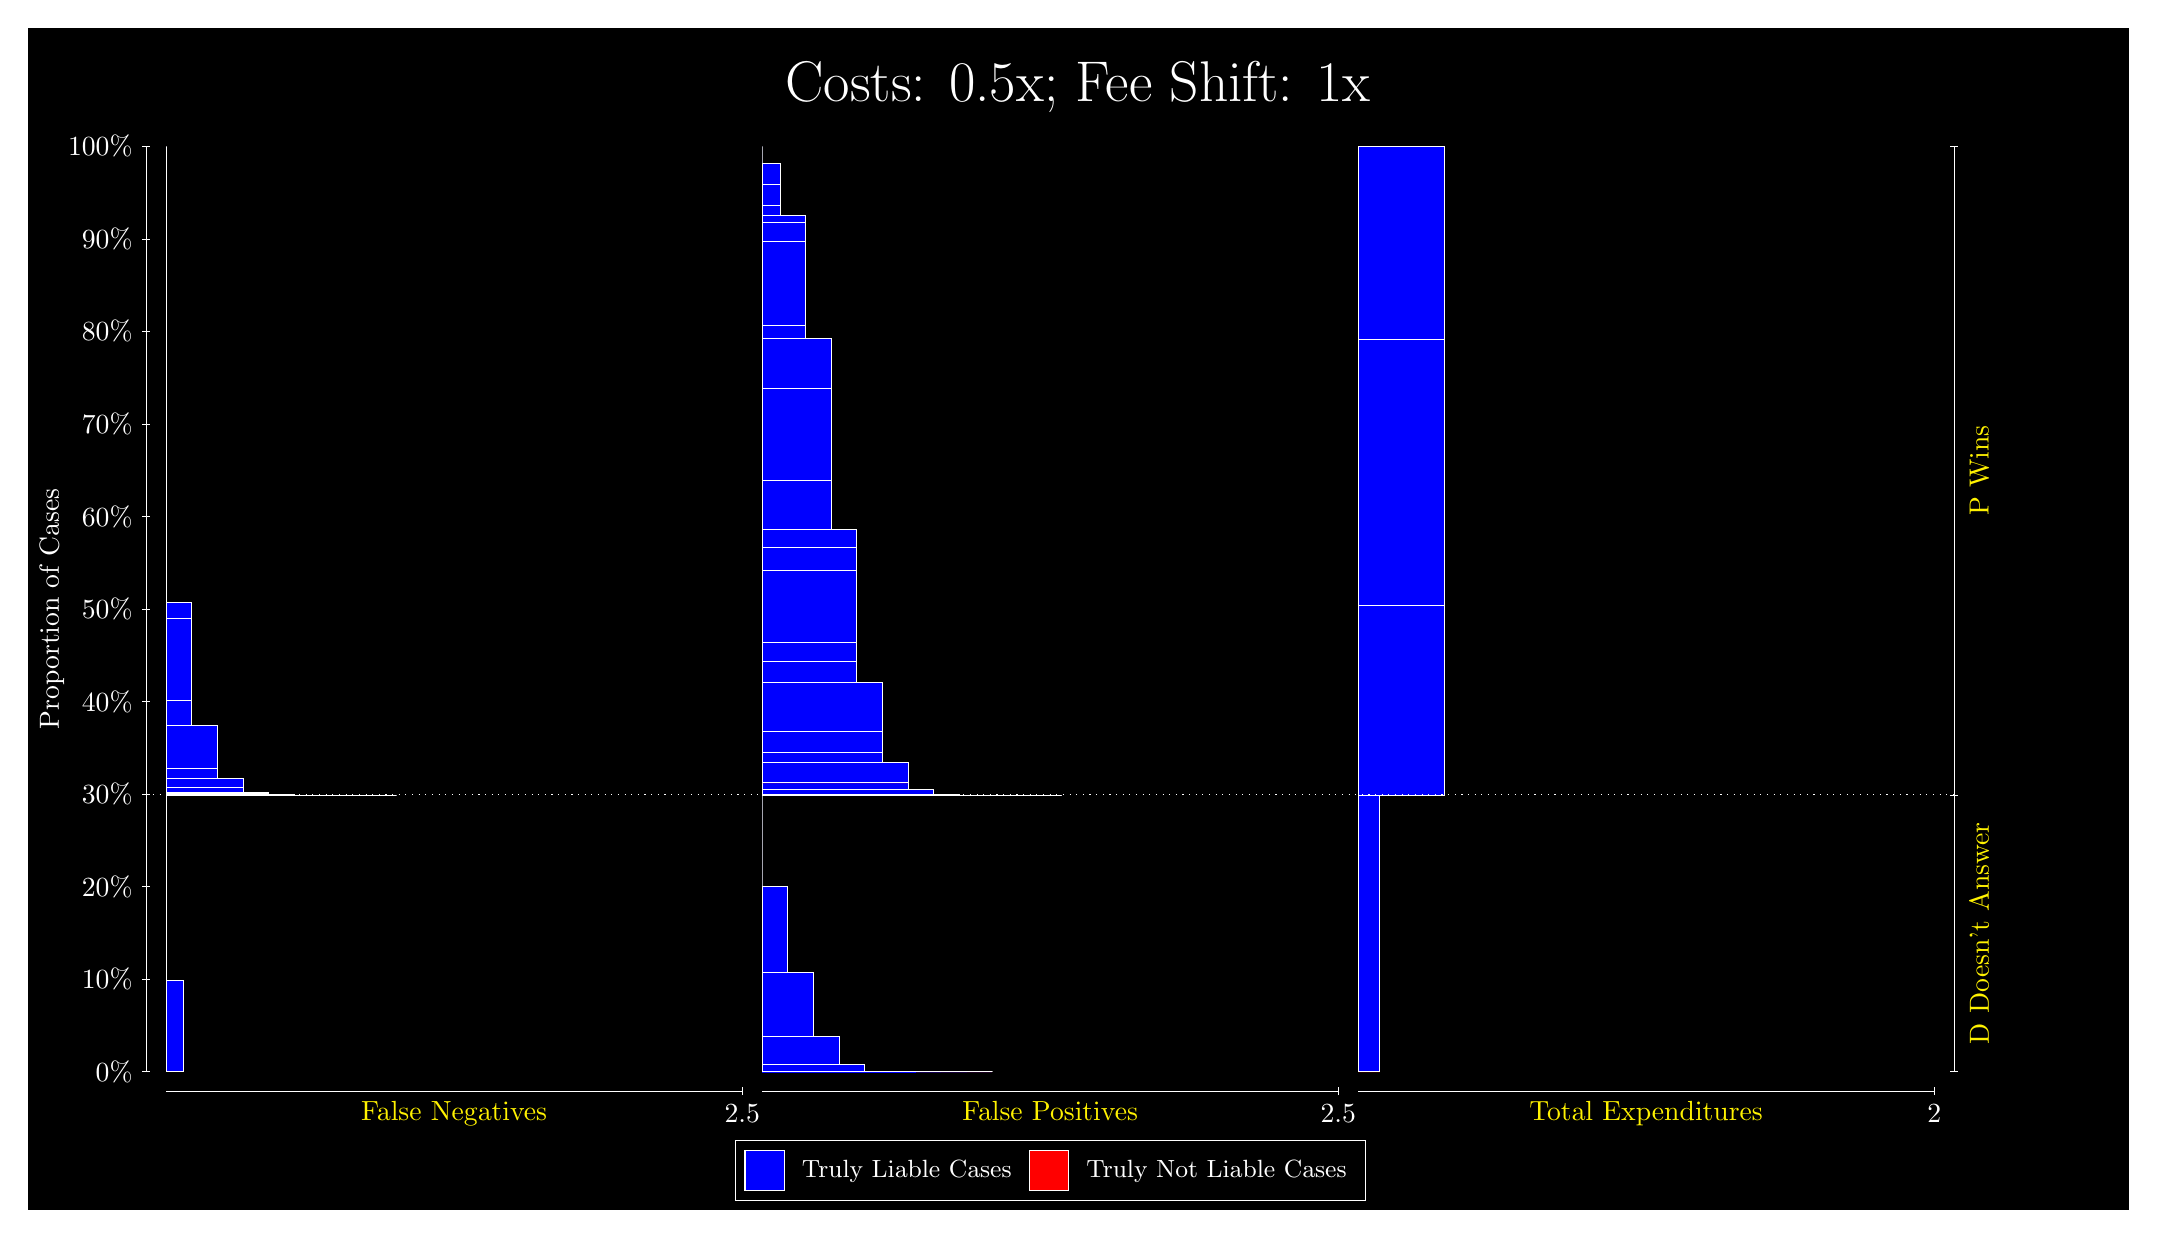
\begin{tikzpicture}
\draw[fill=black] (0,0) rectangle (26.667,15);
\draw[text=white] (0,13.5) rectangle (26.667,15) node[midway] {\huge Costs: 0.5x; Fee Shift: 1x};
\draw[white, very thin] (1.5,1.75) -- (1.5,13.5);
\node[rotate=90, text=white, anchor=center] at (0.3, 7.625) {Proportion of Cases};
\draw[white, very thin] (1.45,1.75) -- (1.55,1.75);
\node[text=white, anchor=east] at (1.45, 1.75) {0\%};
\draw[white, very thin] (1.45,2.925) -- (1.55,2.925);
\node[text=white, anchor=east] at (1.45, 2.925) {10\%};
\draw[white, very thin] (1.45,4.1) -- (1.55,4.1);
\node[text=white, anchor=east] at (1.45, 4.1) {20\%};
\draw[white, very thin] (1.45,5.275) -- (1.55,5.275);
\node[text=white, anchor=east] at (1.45, 5.275) {30\%};
\draw[white, very thin] (1.45,6.45) -- (1.55,6.45);
\node[text=white, anchor=east] at (1.45, 6.45) {40\%};
\draw[white, very thin] (1.45,7.625) -- (1.55,7.625);
\node[text=white, anchor=east] at (1.45, 7.625) {50\%};
\draw[white, very thin] (1.45,8.8) -- (1.55,8.8);
\node[text=white, anchor=east] at (1.45, 8.8) {60\%};
\draw[white, very thin] (1.45,9.975) -- (1.55,9.975);
\node[text=white, anchor=east] at (1.45, 9.975) {70\%};
\draw[white, very thin] (1.45,11.15) -- (1.55,11.15);
\node[text=white, anchor=east] at (1.45, 11.15) {80\%};
\draw[white, very thin] (1.45,12.325) -- (1.55,12.325);
\node[text=white, anchor=east] at (1.45, 12.325) {90\%};
\draw[white, very thin] (1.45,13.5) -- (1.55,13.5);
\node[text=white, anchor=east] at (1.45, 13.5) {100\%};

\draw[white, very thin] (24.457,1.75) -- (24.457,13.5);
\draw[white, very thin] (24.407,1.75) -- (24.507,1.75);
\node[anchor=west] at (24.407, 1.75) {};
\draw[white, very thin] (24.407,5.264) -- (24.507,5.264);
\node[anchor=west] at (24.407, 5.264) {};
\draw[white, very thin] (24.407,13.5) -- (24.507,13.5);
\node[anchor=west] at (24.407, 13.5) {};

\draw[white, very thin, fill=blue] (1.75,1.75) rectangle (1.9696,2.9145);
\draw[white, very thin, fill=red] (1.75,2.9145) rectangle (1.75,2.9145);
\draw[white, very thin, fill=blue] (1.75,2.9145) rectangle (1.75,5.264);
\draw[white, very thin, fill=blue] (1.75,5.264) rectangle (4.6775,5.264);
\draw[white, very thin, fill=blue] (1.75,5.264) rectangle (4.3523,5.264);
\draw[white, very thin, fill=blue] (1.75,5.264) rectangle (4.027,5.264);
\draw[white, very thin, fill=blue] (1.75,5.264) rectangle (4.027,5.264);
\draw[white, very thin, fill=blue] (1.75,5.264) rectangle (3.7017,5.264);
\draw[white, very thin, fill=blue] (1.75,5.264) rectangle (3.7017,5.2642);
\draw[white, very thin, fill=blue] (1.75,5.2642) rectangle (3.3764,5.2671);
\draw[white, very thin, fill=blue] (1.75,5.2671) rectangle (3.0511,5.2797);
\draw[white, very thin, fill=blue] (1.75,5.2797) rectangle (3.0511,5.2975);
\draw[white, very thin, fill=blue] (1.75,5.2975) rectangle (2.7258,5.3544);
\draw[white, very thin, fill=blue] (1.75,5.3544) rectangle (2.7258,5.475);
\draw[white, very thin, fill=blue] (1.75,5.475) rectangle (2.7258,5.4788);
\draw[white, very thin, fill=blue] (1.75,5.4788) rectangle (2.4006,5.6005);
\draw[white, very thin, fill=blue] (1.75,5.6005) rectangle (2.4006,6.1449);
\draw[white, very thin, fill=blue] (1.75,6.1449) rectangle (2.0753,6.4607);
\draw[white, very thin, fill=blue] (1.75,6.4607) rectangle (2.0753,7.5117);
\draw[white, very thin, fill=blue] (1.75,7.5117) rectangle (2.0753,7.7058);
\draw[white, very thin, fill=red] (1.75,7.7058) rectangle (1.75,7.7058);
\draw[white, very thin, fill=blue] (1.75,7.7058) rectangle (1.75,13.5);
\draw[white, very thin, fill=red] (9.3189,1.75) rectangle (12.246,1.75);
\draw[white, very thin, fill=blue] (9.3189,1.75) rectangle (12.246,1.75);
\draw[white, very thin, fill=blue] (9.3189,1.75) rectangle (11.921,1.75);
\draw[white, very thin, fill=blue] (9.3189,1.75) rectangle (11.596,1.75);
\draw[white, very thin, fill=blue] (9.3189,1.75) rectangle (11.271,1.7503);
\draw[white, very thin, fill=blue] (9.3189,1.7503) rectangle (10.945,1.7576);
\draw[white, very thin, fill=blue] (9.3189,1.7576) rectangle (10.62,1.8361);
\draw[white, very thin, fill=blue] (9.3189,1.8361) rectangle (10.295,2.1984);
\draw[white, very thin, fill=blue] (9.3189,2.1984) rectangle (9.9694,3.0086);
\draw[white, very thin, fill=blue] (9.3189,3.0086) rectangle (9.6442,4.0995);
\draw[white, very thin, fill=blue] (9.3189,4.0995) rectangle (9.3189,5.264);
\draw[white, very thin, fill=red] (9.3189,5.264) rectangle (13.125,5.264);
\draw[white, very thin, fill=blue] (9.3189,5.264) rectangle (13.125,5.264);
\draw[white, very thin, fill=red] (9.3189,5.264) rectangle (12.799,5.264);
\draw[white, very thin, fill=blue] (9.3189,5.264) rectangle (12.799,5.264);
\draw[white, very thin, fill=blue] (9.3189,5.264) rectangle (12.474,5.264);
\draw[white, very thin, fill=red] (9.3189,5.264) rectangle (12.474,5.264);
\draw[white, very thin, fill=blue] (9.3189,5.264) rectangle (12.474,5.264);
\draw[white, very thin, fill=blue] (9.3189,5.264) rectangle (12.149,5.2642);
\draw[white, very thin, fill=blue] (9.3189,5.2642) rectangle (12.149,5.2643);
\draw[white, very thin, fill=red] (9.3189,5.2643) rectangle (12.149,5.2643);
\draw[white, very thin, fill=blue] (9.3189,5.2643) rectangle (12.149,5.2647);
\draw[white, very thin, fill=red] (9.3189,5.2647) rectangle (11.824,5.2647);
\draw[white, very thin, fill=blue] (9.3189,5.2647) rectangle (11.824,5.2699);
\draw[white, very thin, fill=blue] (9.3189,5.2699) rectangle (11.824,5.2714);
\draw[white, very thin, fill=blue] (9.3189,5.2714) rectangle (11.824,5.2731);
\draw[white, very thin, fill=red] (9.3189,5.2731) rectangle (11.498,5.2731);
\draw[white, very thin, fill=blue] (9.3189,5.2731) rectangle (11.498,5.3299);
\draw[white, very thin, fill=blue] (9.3189,5.3299) rectangle (11.498,5.3404);
\draw[white, very thin, fill=blue] (9.3189,5.3404) rectangle (11.173,5.4184);
\draw[white, very thin, fill=red] (9.3189,5.4184) rectangle (11.173,5.4184);
\draw[white, very thin, fill=blue] (9.3189,5.4184) rectangle (11.173,5.6734);
\draw[white, very thin, fill=blue] (9.3189,5.6734) rectangle (10.848,5.8049);
\draw[white, very thin, fill=blue] (9.3189,5.8049) rectangle (10.848,6.0751);
\draw[white, very thin, fill=red] (9.3189,6.0751) rectangle (10.848,6.0751);
\draw[white, very thin, fill=blue] (9.3189,6.0751) rectangle (10.848,6.688);
\draw[white, very thin, fill=blue] (9.3189,6.688) rectangle (10.522,6.9555);
\draw[white, very thin, fill=blue] (9.3189,6.9555) rectangle (10.522,7.2056);
\draw[white, very thin, fill=red] (9.3189,7.2056) rectangle (10.522,7.2056);
\draw[white, very thin, fill=blue] (9.3189,7.2056) rectangle (10.522,8.1122);
\draw[white, very thin, fill=blue] (9.3189,8.1122) rectangle (10.522,8.4066);
\draw[white, very thin, fill=blue] (9.3189,8.4066) rectangle (10.522,8.6381);
\draw[white, very thin, fill=blue] (9.3189,8.6381) rectangle (10.197,9.2606);
\draw[white, very thin, fill=red] (9.3189,9.2606) rectangle (10.197,9.2606);
\draw[white, very thin, fill=blue] (9.3189,9.2606) rectangle (10.197,10.422);
\draw[white, very thin, fill=blue] (9.3189,10.422) rectangle (10.197,11.058);
\draw[white, very thin, fill=blue] (9.3189,11.058) rectangle (9.8718,11.231);
\draw[white, very thin, fill=blue] (9.3189,11.231) rectangle (9.8718,12.288);
\draw[white, very thin, fill=blue] (9.3189,12.288) rectangle (9.8718,12.538);
\draw[white, very thin, fill=blue] (9.3189,12.538) rectangle (9.8718,12.619);
\draw[white, very thin, fill=blue] (9.3189,12.619) rectangle (9.5466,12.753);
\draw[white, very thin, fill=blue] (9.3189,12.753) rectangle (9.5466,13.021);
\draw[white, very thin, fill=blue] (9.3189,13.021) rectangle (9.5466,13.285);
\draw[white, very thin, fill=blue] (9.3189,13.285) rectangle (9.3189,13.5);
\draw[white, very thin, fill=red] (16.888,1.75) rectangle (17.162,1.75);
\draw[white, very thin, fill=blue] (16.888,1.75) rectangle (17.162,5.264);
\draw[white, very thin, fill=red] (16.888,5.264) rectangle (17.986,5.264);
\draw[white, very thin, fill=blue] (16.888,5.264) rectangle (17.986,7.6726);
\draw[white, very thin, fill=red] (16.888,7.6726) rectangle (17.986,7.6726);
\draw[white, very thin, fill=blue] (16.888,7.6726) rectangle (17.986,11.049);
\draw[white, very thin, fill=red] (16.888,11.049) rectangle (17.986,11.049);
\draw[white, very thin, fill=blue] (16.888,11.049) rectangle (17.986,13.5);
\draw[white, dotted] (1.5,5.264) -- (24.457,5.264);
\draw[white, very thin] (1.75,1.5) -- (9.0689,1.5);
\node[text=yellow, anchor=north] at (5.4094, 1.5) {False Negatives};
\draw[white, very thin] (9.0689,1.45) -- (9.0689,1.55);
\node[text=white, anchor=north] at (9.0689, 1.45) {2.5};

\draw[white, very thin] (9.3189,1.5) -- (16.638,1.5);
\node[text=yellow, anchor=north] at (12.978, 1.5) {False Positives};
\draw[white, very thin] (16.638,1.45) -- (16.638,1.55);
\node[text=white, anchor=north] at (16.638, 1.45) {2.5};

\draw[white, very thin] (16.888,1.5) -- (24.207,1.5);
\node[text=yellow, anchor=north] at (20.547, 1.5) {Total Expenditures};
\draw[white, very thin] (24.207,1.45) -- (24.207,1.55);
\node[text=white, anchor=north] at (24.207, 1.45) {2};

\node[text=yellow, centered, rotate=90] at (24.777, 3.507) {D Doesn't Answer};
\node[text=yellow, centered, rotate=90] at (24.777, 9.382) {P Wins};

\draw (12.978300999999998,1.5) node[draw=none] (baseCoordinate) {};
\begin{scope}[align=center]
        \matrix[scale=0.5, draw=white, below=0.5cm of baseCoordinate, nodes={draw}, column sep=0.1cm]{
            \node[rectangle, draw, minimum width=0.5cm, minimum height=0.5cm, fill=blue] {}; &
            \node[draw=none, font=\small, text=white] (B) {Truly Liable Cases}; &
            \node[rectangle, draw, minimum width=0.5cm, minimum height=0.5cm, fill=red] {}; &
            \node[draw=none, font=\small, text=white] (B) {Truly Not Liable Cases}; \\
            };
\end{scope}

\end{tikzpicture}
\end{document}